% !TEX program = pdflatex
% =====================================================================
%  MCM/ICM (COMAP) paper template -- single self-contained file
%  Files needed: main.tex + refs.bib (nothing else; no shared preamble).
% ---------------------------------------------------------------------
%  Build (run once, then again for cross-references, then again for the
%  bibliography--the bibliography needs one bibtex pass):
%      pdflatex main.tex
%      bibtex   main
%      pdflatex main.tex
%      pdflatex main.tex
%  One-liner: latexmk -pdf main.tex
%  Compiler: pdfLaTeX (plain English document; NO CJK package is loaded,
%  and none may be added -- a Chinese font package would break the
%  English-only requirement and is not needed here).
%
%  BEFORE YOU WRITE: read the current year's official instructions.
%  https://www.contest.comap.com/undergraduate/contests/mcm/instructions.html
%  Rules are revised every year; the statements below are the ones
%  recorded in references/contests.md and are annotated with their year:
%   (a) 25-PAGE LIMIT applies to the WHOLE submission: Summary Sheet,
%       table of contents, body, references, notes, APPENDICES AND CODE,
%       plus any problem-specific requirements. (2027 rules wording;
%       the limit is the same in the 2026 rules.) The "Report on Use of
%       AI" is the only part placed AFTER the 25-page solution and does
%       NOT count toward the limit.
%   (b) One Adobe PDF, in English, font size at least 12 pt.
%   (c) EVERY page must carry the team control number and the page number
%       in the header, e.g. "Team # 0000000, Page 6 of 25" -- see the
%       fancyhdr setup below.
%   (d) Page 1 is the Summary Sheet (COMAP publishes a Word/LaTeX version
%       of it each year; use that if you prefer its exact layout).
%   (e) Names of team members, advisor and school must NOT appear on any
%       page; only the control number is allowed. That is why this
%       template has no \author, no \maketitle and no title block.
%   (f) Submit one PDF named <control number>.pdf, attachment < 25 MB.
%       Do not send programs or data files -- judges do not use them.
%   (g) DO NOT add a Chinese/CJK package to this file: the submission must
%       be English.
%
%  Structure implemented below (follows references/paper-structure.md):
%      1  Summary Sheet (page 1, single page, 12 pt)
%      2  Table of Contents (optional; COUNTS toward the 25 pages)
%      3  Introduction
%      4  Assumptions and Justifications
%      5  Notations
%      6  Model Development
%      7  Results
%      8  Sensitivity Analysis
%      9  Strengths and Weaknesses
%     10  Conclusion
%     11  References
%     12  Report on Use of AI          <- after the 25-page solution, not counted
%     13  Appendices (code)            <- COUNTED in the 25 pages
%     14  Memo / Letter                <- only if the problem asks for it
% =====================================================================

\documentclass[12pt]{article}

% ------------------------- layout -------------------------
\usepackage[letterpaper,margin=1in,headheight=15pt]{geometry}
% The rules fix the minimum font size (12 pt) but do not prescribe
% margins; 1 in margins are a common, safe choice.
\usepackage[T1]{fontenc}          % T1: correct < > and better hyphenation
\usepackage{lmodern}              % scalable Latin Modern fonts for pdfLaTeX

% ------------------------- math -------------------------
\usepackage{amsmath}
\usepackage{amssymb}
\usepackage{bm}

% ------------------------- tables and figures -------------------------
\usepackage{booktabs}             % three-line tables
\usepackage{multirow}
\usepackage{array}
\usepackage{tabularx}
\usepackage{graphicx}
\usepackage{float}
\usepackage{caption}
\usepackage{tikz}                 % draw the flow chart yourself: no borrowed images
\usetikzlibrary{arrows.meta,positioning}
\usepackage{pgfplots}             % demo figure only; export your own plots to PDF
\pgfplotsset{compat=1.18}

% ------------------------- pseudocode -------------------------
\usepackage{algorithm}
\usepackage{algpseudocode}

% ------------------------- code listings -------------------------
\usepackage{listings}
\usepackage{xcolor}
\definecolor{codekw}{RGB}{0,0,180}
\definecolor{codecmt}{RGB}{0,128,0}
\definecolor{codestr}{RGB}{160,32,32}
\definecolor{codebg}{RGB}{248,248,248}
\lstset{
  language=Python,
  basicstyle=\ttfamily\small,
  keywordstyle=\color{codekw}\bfseries,
  commentstyle=\color{codecmt},
  stringstyle=\color{codestr},
  numbers=left,
  numberstyle=\tiny\color{gray},
  numbersep=6pt,
  frame=single,
  rulecolor=\color{gray!50},
  backgroundcolor=\color{codebg},
  breaklines=true,
  postbreak=\mbox{\textcolor{gray}{$\hookrightarrow$}\space},
  columns=flexible,
  keepspaces=true,
  showstringspaces=false,
  tabsize=4,
  captionpos=t,
  xleftmargin=1.5em,
  aboveskip=1em,belowskip=1em
}

% ------------------------- bibliography -------------------------
\usepackage[numbers,sort&compress]{natbib}

% ------------- running header: control number + page number -------------
\usepackage{fancyhdr}
\usepackage{lastpage}
\newcommand{\teamcontrol}{XXXXXXX}   % <-- REPLACE with your team control number
\pagestyle{fancy}
\fancyhf{}
% Requirement: every page shows the control number and the page number.
% "Page X of Y" is produced with lastpage, so run pdflatex twice.
\fancyhead[C]{\small Team \# \teamcontrol, Page \thepage\ of \pageref{LastPage}}
\renewcommand{\headrulewidth}{0.4pt}
\renewcommand{\footrulewidth}{0pt}

\captionsetup{font=small,labelsep=quad}

% =====================================================================
\begin{document}

% =====================================================================
%  PAGE 1 -- SUMMARY SHEET
%  * single page, at the very front, at least 12 pt
%  * no title/team/adviser/school block at the top of the page: the
%    control number lives in the running header only
%  * write it LAST and revise it several times. COMAP's own writing guide:
%    "judges place considerable weight on the summary, and winning papers
%    are often distinguished from other papers based on the quality of
%    the summary." A summary that merely restates the problem is weak.
%  * every task must appear with a QUANTITATIVE result and how it was
%    validated; add one sentence on sensitivity and one on
%    strengths/limitations. 250-400 words is a good target.
% =====================================================================
\thispagestyle{fancy}
\begin{center}
  {\large\bfseries Summary}
\end{center}

<One or two sentences: what we are asked to do, for whom, and why it matters.>

For Task 1, we develop a <model type> model. We assume <key assumption> and
formulate <objective / governing equations in one compact sentence>. Using
<method and tool>, we find <quantitative result with units>. This result
<agrees with / differs from> <benchmark> by <x%>.

For Task 2, we extend the model by introducing <new mechanism or variable>.
Solving with <method> gives <quantitative finding>, a <x%> change relative to
<baseline>.

We then test the assumptions of the model. Varying <parameter> by $\pm 20\%$
changes <output> by less than <y%>, so <the recommendation is robust / the
model is sensitive to this parameter and it must be measured accurately>.

Finally, we give a concrete, decision-relevant recommendation. Our main
strengths are <strength>; the main limitations are <limitation>, which we
would address by <next step>.

\vspace{0.6em}
\noindent\textbf{Keywords:} <model>; <method>; <application>

\newpage

% =====================================================================
%  TABLE OF CONTENTS -- OPTIONAL
%  A table of contents is recommended by COMAP's writing guide, but its
%  pages COUNT toward the 25-page limit. Uncomment only if you have room.
% =====================================================================
% \tableofcontents
% \newpage

\section{Introduction}
Restate the problem in your own words -- do NOT copy the problem statement.
Show that you understand it: state the context, what is given, what is asked,
and what a useful answer looks like~\cite{giordano2014mathematical}.

<Background, players/stakeholders, data available, and the deliverables you
produce for each task.>

\section{Assumptions and Justifications}
Every assumption must carry a justification and a statement of its impact on
the model; unsupported assumptions are one of the fastest ways to lose
points. Three to six assumptions is typical.

\begin{enumerate}
  \item \textbf{Assumption 1:} <content>.
        \emph{Justification:} <evidence, data or a cited source>.
        \emph{Impact:} <what it changes in the model>.
  \item \textbf{Assumption 2:} <content>.
        \emph{Justification:} <...>. \emph{Impact:} <...>.
  \item \textbf{Assumption 3:} <content>.
        \emph{Justification:} <...>. \emph{Impact:} <...>.
\end{enumerate}

\section{Notations}
\begin{table}[htbp]
  \centering
  \caption{Notation used throughout the paper}
  \label{tab:notation}
  \begin{tabular}{clc}
    \toprule
    Symbol & Meaning & Unit \\
    \midrule
    $x_{ij}$ & Decision variable: <meaning> & <unit> \\
    $c_{ij}$ & <meaning>                  & <unit> \\
    $Z$      & Objective value            & <unit> \\
    $\lambda$& <meaning, e.g. weight>     & --     \\
    \bottomrule
  \end{tabular}
\end{table}

Table~\ref{tab:notation} lists the symbols used below; every symbol is defined
again where it first appears.

\section{Model Development}
For each task: why this model (and why not the alternatives), the
mathematical formulation, the solution algorithm, and the results.

\subsection{Task 1: <model name>}

\subsubsection{Model choice}
<Motivation and comparison with alternatives: e.g. the decision mixes
discrete and continuous variables, so a mixed-integer program is preferred
over a pure linear program~\cite{boyd2004convex}; a multi-objective variant
can be handled with an evolutionary algorithm~\cite{deb2002nsga2}.>

\subsubsection{Mathematical formulation}
\begin{align}
  \min\ Z & = \sum_{i \in V}\sum_{j \in J} c_{ij} x_{ij}
             + \lambda \sum_{j \in J} f_j y_j \label{eq:objective} \\[2pt]
  \text{s.t.}\quad
  & \sum_{j \in J} x_{ij} = d_i, \qquad \forall i \in V, \label{eq:demand} \\[2pt]
  & \sum_{i \in V} x_{ij} \le M y_j, \qquad \forall j \in J, \label{eq:link} \\[2pt]
  & x_{ij} \ge 0,\quad y_j \in \{0,1\}. \label{eq:domain}
\end{align}
Equation~\eqref{eq:objective} is the objective; \eqref{eq:demand} enforces
demand satisfaction; \eqref{eq:link} is the fixed-charge linking constraint
($M$ large enough); \eqref{eq:domain} gives the ranges. The model is valid
under <conditions>, and it does not apply when <limitation>.

\subsubsection{Solution algorithm}
\begin{algorithm}[H]
  \caption{<Algorithm name> for Task 1}
  \label{alg:task1}
  \begin{algorithmic}[1]
    \Require demands $\{d_i\}$, candidate sites $J$, cost matrix $(c_{ij})$,
             iteration cap $K$
    \Ensure  site selection $y^{*}$ and objective value $Z^{*}$
    \State initialize $y^{(0)}$ by <construction rule>, $Z^{(0)} \gets +\infty$
    \For{$k = 1$ \textbf{to} $K$}
      \State fix $y^{(k-1)}$, solve \eqref{eq:demand}--\eqref{eq:link}
             for the flow $x^{(k)}$
      \State build the neighbourhood $\mathcal{N}(y^{(k-1)})$ by <move>
      \If{$\exists\, y' \in \mathcal{N}(y^{(k-1)})$ with $Z(y') < Z^{(k-1)}$}
        \State $y^{(k)} \gets \arg\min_{y' \in \mathcal{N}} Z(y')$
      \Else
        \State $y^{(k)} \gets y^{(k-1)}$; \textbf{break}
      \EndIf
    \EndFor
    \State \Return $y^{(K)},\, Z^{(K)}$
  \end{algorithmic}
\end{algorithm}

Algorithm~\ref{alg:task1} runs in <O(.)> time. Parameters:
<step size / penalty / iteration cap>; convergence criterion: <criterion>.
Software: <Python 3.11 + numpy 1.26 / Gurobi 11 / MATLAB R2023b>.

\subsubsection{Results}
% PLACEHOLDER DATA: the coordinates below only demonstrate the layout.
% Replace them with your own computed series.
\begin{figure}[htbp]
  \centering
  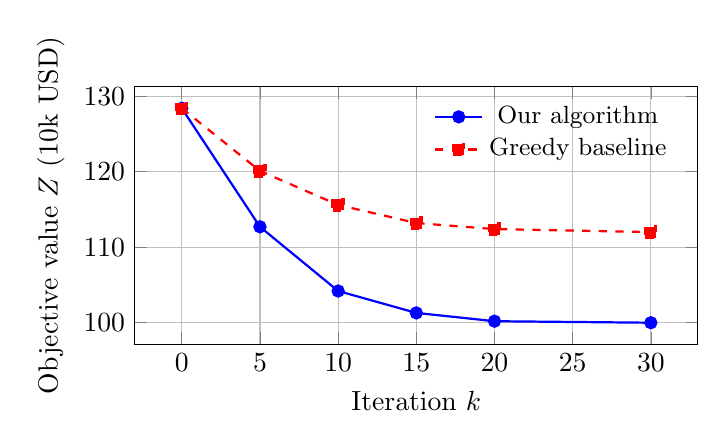
\begin{tikzpicture}
    \begin{axis}[
        width=0.72\textwidth, height=0.40\textwidth,
        xlabel={Iteration $k$},
        ylabel={Objective value $Z$ (10k USD)},
        grid=major,
        legend pos=north east,
        legend style={font=\small, draw=none, fill=none},
        every axis plot/.append style={thick}
      ]
      \addplot[mark=*, color=blue] coordinates
        {(0,128.4)(5,112.7)(10,104.2)(15,101.3)(20,100.2)(30,100.0)};
      \addlegendentry{Our algorithm}
      \addplot[mark=square*, dashed, color=red] coordinates
        {(0,128.4)(5,120.1)(10,115.6)(15,113.2)(20,112.4)(30,112.0)};
      \addlegendentry{Greedy baseline}
    \end{axis}
  \end{tikzpicture}
  \caption{Convergence of our algorithm against the greedy baseline
           (x-axis: iteration; y-axis: objective value, 10k USD)}
  \label{fig:convergence}
\end{figure}

\begin{table}[htbp]
  \centering
  \caption{Task 1 results (placeholder values -- replace with program output)}
  \label{tab:task1}
  \begin{tabular}{lcc}
    \toprule
    Scenario & Objective value $Z$ (10k USD) & Coverage (\%) \\
    \midrule
    Current practice (baseline) & 128.4 & 86.5 \\
    Greedy heuristic            & 112.0 & 91.2 \\
    Our model                   & 100.0 & 96.8 \\
    \bottomrule
  \end{tabular}
\end{table}

Figure~\ref{fig:convergence} and Table~\ref{tab:task1} show that our algorithm
converges after <k> iterations and lowers the objective by <x%> relative to
the baseline. All numbers are produced by the code in Appendix~\ref{app:code},
so the paper and the code cannot disagree.

% Draw your own flow chart -- judges use it to see your reasoning in seconds.
\begin{figure}[htbp]
  \centering
  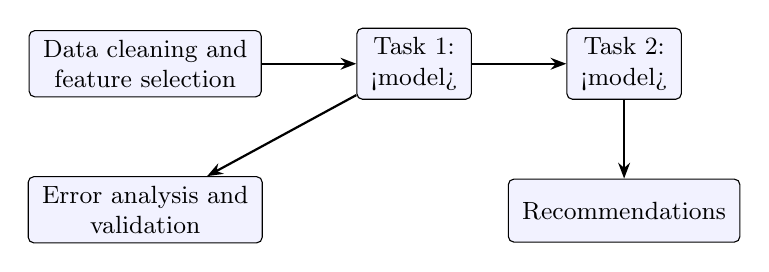
\begin{tikzpicture}[
      node distance=8mm and 10mm,
      every node/.style={font=\small},
      box/.style={draw, rounded corners=2pt, align=center, minimum height=8mm,
                  inner xsep=5pt, fill=blue!5},
      ar/.style={-{Stealth[length=2mm]}, thick}
    ]
    \node[box] (data) {Data cleaning and\\feature selection};
    \node[box, right=12mm of data] (t1) {Task 1:\\<model>};
    \node[box, right=12mm of t1]   (t2) {Task 2:\\<model>};
    \node[box, below=10mm of data] (err) {Error analysis and\\validation};
    \node[box, below=10mm of t2]   (dec) {Recommendations};
    \draw[ar] (data) -- (t1);
    \draw[ar] (t1) -- (t2);
    \draw[ar] (t1) -- (err);
    \draw[ar] (t2) -- (dec);
  \end{tikzpicture}
  \caption{Overall modelling workflow (replace with your own)}
  \label{fig:workflow}
\end{figure}

\subsection{Task 2: <model name>}
<Same four-part structure; emphasise what is new relative to Task 1 and why
the new mechanism is needed.>

\section{Results}
Present the figures and tables that answer each task, and reference every one
of them in the text with an interpretation -- a figure that is never mentioned
adds nothing.

\subsection{Task 1 results}
<Quantitative answer, with units, plus what it means for the decision maker.>

\subsection{Task 2 results}
<...>

\subsection{Comparison with baselines}
<Compare against at least one baseline (current practice, a greedy rule, a
simpler model, or published values) and explain where the improvement comes
from: model structure, solution quality, or data.>

\section{Sensitivity Analysis}
COMAP expects the assumptions of the model to be tested explicitly.

\subsection{Parameter sensitivity}
<Choose the two to four parameters that matter most; state the perturbation
range and why it is realistic ($\pm 10\%/\pm 20\%$, or the precision of the
data). Global sensitivity indices such as Sobol' indices can be used to
allocate the variance~\cite{saltelli2008global}.>

<Closing sentence template: "When <parameter> varies within <range>, <output>
changes by less than <z%>, so the recommendation is robust", or "...the model
is highly sensitive to <parameter>, which must therefore be measured
accurately.">

\subsection{Error and stability analysis}
<Error metric (RMSE/MAE/MAPE), its value, and an explanation of why the error
is of that order (data precision, model simplification, stochastic effects).
Also test extreme or degenerate cases.>

\section{Strengths and Weaknesses}
Both are required; listing only strengths reads as an incomplete analysis.

\subsection{Strengths}
\begin{itemize}
  \item <strength 1, tied to a verifiable fact>
  \item <strength 2>
  \item <strength 3>
\end{itemize}

\subsection{Weaknesses and how we would fix them}
\begin{itemize}
  \item <limitation 1> $\rightarrow$ <next step>.
  \item <limitation 2> $\rightarrow$ <next step>.
\end{itemize}

\section{Conclusion}
Answer every question that was asked, with numbers and units.

For Task 1, we recommend <decision> because <numerical support>. For Task 2,
<decision and support>. Because <parameter> is the dominant source of
uncertainty, we would <monitoring or robustness action>.

% =====================================================================
%  REFERENCES
%  References COUNT toward the 25-page limit. Cite everything you used,
%  including web pages (with an access date). ai.bib entries for tools you
%  used belong here too -- they must also appear in the Report on Use of AI.
% =====================================================================
\bibliographystyle{unsrtnat}
\bibliography{refs}

% =====================================================================
%  REPORT ON USE OF AI
%  * COMAP policy: if you used any AI tool you must (i) cite it inline and
%    list it in the references, and (ii) attach this report.
%  * Placement: AFTER the 25-page solution. It does NOT count toward the
%    25-page limit (it is the only such part).
%  * You must verify AI-generated content and citations and correct the
%    errors; undisclosed AI text can be treated as plagiarism and lead to
%    disqualification. Use AI cautiously for model choice and construction,
%    code generation, interpretation of results and scientific conclusions.
% =====================================================================
\newpage
\section*{Report on Use of AI}

% --- Case 1: no AI was used ---
We did not use AI tools in this work.

% --- Case 2: AI was used (delete the sentence above and fill this in) ---
% Tool: <name and version/model, e.g. "ChatGPT, GPT-4o">
%   Developer: <...>; Date of release/version used: <...>.
% Purpose: <e.g. literature search, code debugging, language editing>.
% How it was used: <prompts and workflow, with one or two typical exchanges>.
% Verification: <what we checked, what we corrected, and who on the team
%   verified it. For code: how we confirmed it reproduces our numbers.>
% Inline citations to this report appear at <section/equation numbers>.

% =====================================================================
%  APPENDICES
%  WARNING: appendices, code and any supplementary derivations are part of
%  the submission and COUNT toward the 25-page limit. Keep them lean.
% =====================================================================
\appendix
\section{Derivations and supplementary tables}
\label{app:derivations}
<Long proofs, extra tables, additional parameter values. Put anything that
would otherwise break the flow of the body here, but mind the page limit.>

\section{Code}
\label{app:code}
% Recommended: include the real file so the paper and the code cannot drift:
%   \lstinputlisting[language=Python, caption={model.py}]{code/model.py}
% The listing below is a self-contained example, replace it with your code.

\begin{lstlisting}[caption={Example program: least-squares fit with reproducible output}, label={lst:example}]
# -*- coding: utf-8 -*-
"""Example only: fit a quadratic and write results.json.

Environment: Python 3.9+, numpy only.
Every number in the paper should come from a file like this one, never
from a hand-copied value.
"""

import json

import numpy as np


def fit_poly(x, y, degree):
    """Least-squares polynomial fit; returns coefficients (ascending order)."""
    design = np.vander(np.asarray(x, dtype=float), degree + 1)
    coef, *_ = np.linalg.lstsq(design, np.asarray(y, dtype=float), rcond=None)
    return coef


def main():
    rng = np.random.default_rng(20260129)   # fixed seed: reproducible
    x = np.linspace(0.0, 10.0, 60)
    y = 2.0 + 0.8 * x - 0.05 * x ** 2 + rng.normal(0.0, 0.1, x.size)
    coef = fit_poly(x, y, 2)
    y_hat = np.vander(x, 3) @ coef
    rmse = float(np.sqrt(np.mean((y - y_hat) ** 2)))
    with open("results.json", "w", encoding="utf-8") as fp:
        json.dump({"coef": coef.tolist(), "rmse": rmse}, fp, indent=2)
    print("RMSE = %.4f" % rmse)


if __name__ == "__main__":
    main()
\end{lstlisting}

% =====================================================================
%  MEMO / LETTER -- PLACEHOLDER SECTION
%  A memo or letter to a named recipient is required by SOME problems
%  (often 1-2 pages) and not by others: READ THE PROBLEM STATEMENT FIRST
%  and delete this section if it is not required. If it is required, it is
%  part of your submitted solution, so it is subject to the 25-page cap
%  (confirm with the current year's instructions).
% =====================================================================
\section*{Memo (delete this section unless the problem asks for one)}
\begin{flushleft}
To: <recipient>\\
From: Team \# \teamcontrol\\
Date: <date>\\
Re: <subject>
\end{flushleft}

<One paragraph executive summary for a non-technical reader: the decision you
recommend, the numbers that support it, and the main caveat.>

\end{document}
